\chapter{Complex Numbers}
\section{Intro}
When simply using real numbers, you cannot always get the right answer to a given equation. An example of this could be the equation $x^2=-1$. Therefore sometimes we have to use a different number system, which uses the number $i$. 
\begin{align*}
i=\sqrt{-1}
\end{align*}
When squared the number $i$ becomes:
\begin{align*}
i^2=-1
\end{align*}
With the power to the third:
\begin{align*}
i^3=-i
\end{align*}
and with the power to the fourth:
\begin{align*}
i^4=1
\end{align*}
These first four of $i$ creates a loop, $i$ to the fifth will, therefore, be the same as $i$ to the first, $i$ to the seventh is the same as $i$ to the third \\
By using these complex numbers, you can create infinitely more numbers.  
An example of this is the numbers: $2i$ and $-7i$, these are called pure imaginary numbers. When writing pure imaginary numbers you use the form $bi$, where $b$ is a real number that is not $0$. \\
If you put another part on these imaginary numbers, thus $a+bi$ you get the complex numbers. Example $3+4i$ and $-12i+6$. In this case, $a$ is the real part and $b$, where $i$ is, is the imaginary part. $a$ and $b$ are real numbers. By using this method you can make all pure imaginary numbers into a complex number by writing it like this: $0+3i$. $3i$ does not stand alone anymore and is, therefore, a complex number now. You can also rewrite every real number into a complex by doing this $2+0i$. \\
By using complex numbers you can, therefore, find a solution to any given polynomial equation. \\ 
When plotting complex numbers you use the complex plane. The axes are different from the normal coordinate system, instead of the normal $x$ and $y$-axes, you instead have the real part and the imaginary part as the axes. An example of this is shown in the picture below.
\begin{figure}[H]
\begin{center}
  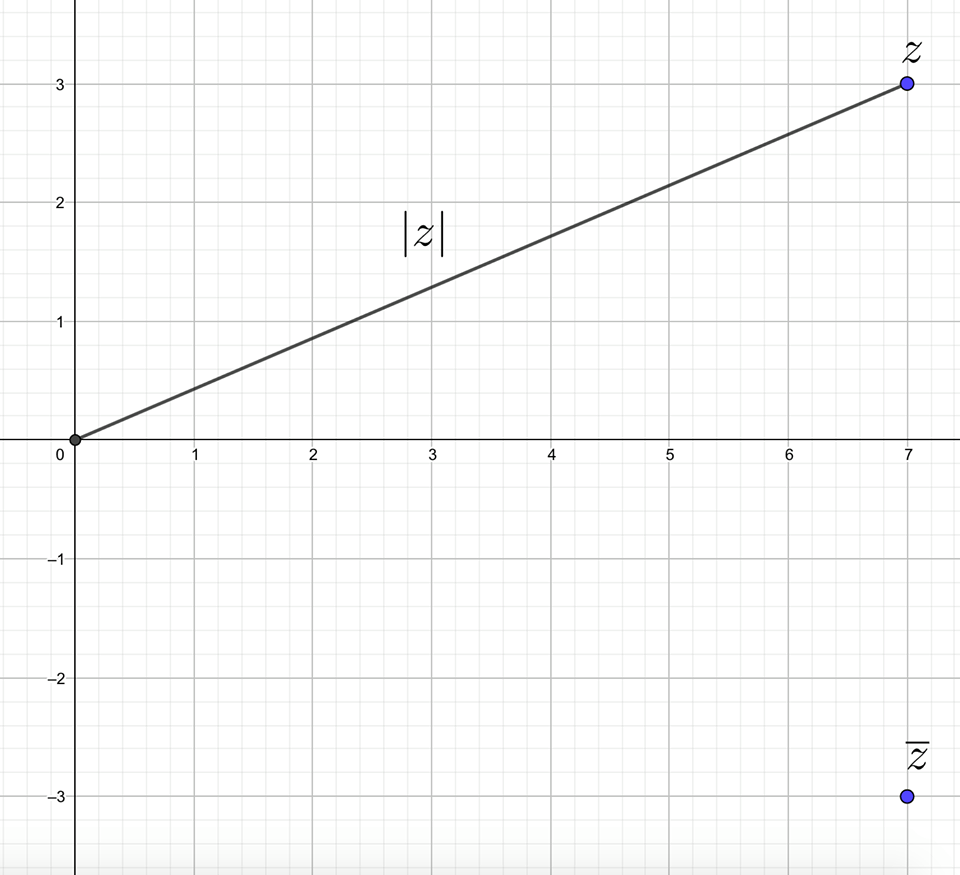
\includegraphics[scale=0.45]{fig/img/complex_plan.png}
   \caption{This shows how to graph the complex number: $7+3i$, on the complex plane.}
   \end{center}
\end{figure}


\section{Adding and Subtracting}
The rules of addition are much like the rules of simply adding two variables of the same type together. For instance, if you have something like $(5+2i)+(9+8i)$ then you can add the complex numbers and the constants and put it together on the general form; $a+bi$. In this case, we get $14+10i$. This rule can be explained in a general form: 
\begin{align*}
(a + bi) + (c + di) = (a + c) + i(b + d)
\end{align*}
Subtracting is similar because you can only subtract a complex number from another complex number, and the same goes for the constants. Here is an example:
\begin{align*}
(21 + 3i) - (2 - 2i) = 21 + 3i - 2 + 2i = 19 + 5i
\end{align*}
Similarly this can be put in a general form:
\begin{align*}
(a + bi) - (c + di) = (a - c) + i(b - d)
\end{align*}
From the examples above we can see that subtracting and adding with complex numbers is identical to subtracting and adding other and more familiar variables such as ($x$, $y$ so on).

\section{Multiplying}
When multiplying with complex numbers it can get a little different than multiplying with other variables, as $i=sqrt(-1)$ , $i^2=-1$ , $i^3=-i$ , $i^4=1$. So if we take an example: \\
\begin{align*}
(3+5i)(4-3i) = 12 - 9i + 20i - 15i^2 = 12 + 11i - 15 \cdot (-1) = 27 + 11i
\end{align*}
The difference is when $x$ is multiplied by $x$ the result is $x^2$, but since there is a definition for $i^2=-1$ the procedure is slightly different. 
This can be described on a general form:
\begin{align*}
(a + bi)(c + di) &= a(c + di) + bi(c + di)
&= ac + adi + bci + bdi^2
&= (ac - bd) + i(ad + bc)
\end{align*}
Since $i^2 = -1$ then $bdi^2$ can be described as $-bd$.

\section{Dividing}
When dividing with a complex number the aim is to get some values we can put on the general form $a + bi$. Here is an example:
\begin{align*}
\frac{18 + 10i}{3 + 2i} &= \frac{(18 + 10i)(3 - 2i)}{(3+2i)(3-2i)} \\[1em]
&= \frac{54 - 36i + 30i - 20i^2}{9 - 9i^2} \\[1em]
&= \frac{54 - 6i - 20 \cdot (-1)}{9 - 9 \cdot (-1)} \\[1em]
&= \frac{74 - 6i}{9 + 9} \\[1em]
&= \frac{74}{18} - \frac{6}{18}i \\[1em]
&= \frac{37}{9} - \frac{1}{3}i
\end{align*}
From the example $\frac{37}{9} - \frac{1}{3}i$ is now on the form $a+bi$ with a and b being fractions. In the example the denominator is being conjugated and as a result of that the imaginary part of the denominator $bi$ disappears and is only left in the numerator. 
This can again be described more generally:
\begin{center}
\begin{align*}
\frac{a + bi}{c + di} 										
&= \frac{(a+bi)(c-di)}{(c+di)(c-di)} 						\\[1em]
&= \frac{a(c-di)+bi(c-di)}{a^2+b^2} 							\\[1em]
&= \frac{ac-adi+bci-bdi^2}{a^2+b^2}							\\[1em]
&= \frac{(ac+bd)+i(bc-ad)}{a^2+b^2}							\\[1em]
&= \frac{ac+bd}{a^2+b^2}+i \frac{bc-ad}{a^2+b^2}				
\end{align*}
\end{center}

\section{The Complex Exponential Equation}
The complex exponential equation derives from Euler’s formula, and is necessary to explain the Laplace transformation. 
%(noget mere tekst)
The complex equation of $z=a+ib$ is:
\begin{align}
e^z=e^{a+ib}=e^ae^{ib}=e^a\cos(b)+i\sin(b)
\end{align}
This function has the property:
$$\mid e^{a+ib} \mid = \mid e^x \mid$$